\begin{center}
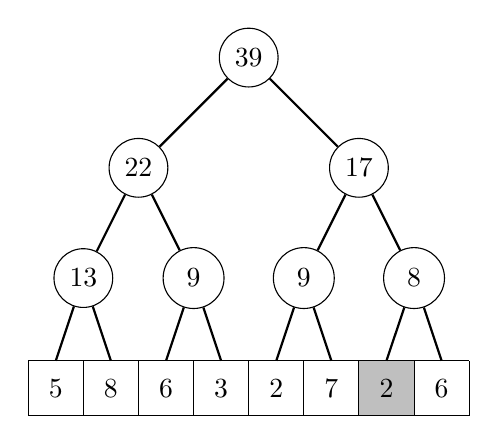
\begin{tikzpicture}[scale=0.7]
\fill[color=lightgray] (6,0) rectangle (7,1);
\draw (0,0) grid (8,1);

\node[anchor=center] at (0.5, 0.5) {5};
\node[anchor=center] at (1.5, 0.5) {8};
\node[anchor=center] at (2.5, 0.5) {6};
\node[anchor=center] at (3.5, 0.5) {3};
\node[anchor=center] at (4.5, 0.5) {2};
\node[anchor=center] at (5.5, 0.5) {7};
\node[anchor=center] at (6.5, 0.5) {2};
\node[anchor=center] at (7.5, 0.5) {6};

\node[draw, circle] (a) at (1,2.5) {13};
\path[draw,thick,-] (a) -- (0.5,1);
\path[draw,thick,-] (a) -- (1.5,1);
\node[draw, circle,minimum size=22pt] (b) at (3,2.5) {9};
\path[draw,thick,-] (b) -- (2.5,1);
\path[draw,thick,-] (b) -- (3.5,1);
\node[draw, circle,minimum size=22pt] (c) at (5,2.5) {9};
\path[draw,thick,-] (c) -- (4.5,1);
\path[draw,thick,-] (c) -- (5.5,1);
\node[draw, circle,minimum size=22pt] (d) at (7,2.5) {8};
\path[draw,thick,-] (d) -- (6.5,1);
\path[draw,thick,-] (d) -- (7.5,1);

\node[draw, circle] (i) at (2,4.5) {22};
\path[draw,thick,-] (i) -- (a);
\path[draw,thick,-] (i) -- (b);
\node[draw, circle] (j) at (6,4.5) {17};
\path[draw,thick,-] (j) -- (c);
\path[draw,thick,-] (j) -- (d);

\node[draw, circle] (m) at (4,6.5) {39};
\path[draw,thick,-] (m) -- (i);
\path[draw,thick,-] (m) -- (j);
\end{tikzpicture}
\end{center}
Actualizaremos la posición 6 del arreglo con el valor 10.